\section{Model} % (fold)
\label{sec:model}

The structure of the data we consider, referred to as \emph{multivariate functional data}, is similar to that presented in \cite{happMultivariateFunctionalPrincipal2018a}. The data consist of independent trajectories of a vector-valued stochastic process $X = (\Xp{1}, \dots, \Xp{P})^\top$, $P\geq 1$. (Here and in the following, for any matrix $A$, $A^\top$ denotes its transpose.) For each $1 \leq p \leq P$, let $\TT{p}$ be a rectangle in some Euclidean space $\RR^{d_p}$ with $d_p \geq 1$, e.g., $\TT{p} = [0,1]^{d_p}$. Each coordinate, or feature, $X^{(p)} : \TT{p} \rightarrow \RR$ is assumed to belong to  $\sLp{\TT{p}}$, the Hilbert space of square-integrable real-valued functions defined on $\TT{p}$, having the usual inner product that we denote by $\inLp{\cdot}{\cdot}$, and $\normLp{\cdot}$ the associated norm. Thus $X$ is a stochastic process indexed by $\pointt = (t_1, \ldots, t_P)$ belonging to the $P-$fold Cartesian product $\TT{} : =\TT{1} \times \cdots \times \TT{P}$ and taking values in the $P-$fold Cartesian product space $\HH \coloneqq \sLp{\TT{1}} \times \dots \times \sLp{\TT{P}}$. 

We consider the function $\inH{\cdot}{\cdot} : \HH \times \HH \rightarrow \RR$,
\begin{equation}\label{eq:innerprodH}
    \inH{f}{g} \coloneqq \sum_{p=1}^{P} \inLp{\fp}{\gp} = \sum_{p=1}^{P}\int_{\TT{p}} \fp(t_p)\gp(t_p) \dd t_p, \quad f, g \in \HH.
\end{equation}
$\HH$ is a Hilbert space with respect to the inner product $\inH{\cdot}{\cdot}$\citep{happMultivariateFunctionalPrincipal2018a}. We denote by $\normH{\cdot}$, the norm induced by $\inH{\cdot}{\cdot}$. Let $\mu : \TT{} \rightarrow \HH$ denote the mean function of the process $X$, $\mu(\pointt) \coloneqq \EE(X(\pointt)),\,\pointt \in \TT{}$. Let $C$ denote the $P \times P$ matrix-valued covariance function which, for $\points, \pointt \in \TT{}$, is defined as
\begin{equation}\label{eq:covariance_function}
    C(\points, \pointt) \coloneqq \EE\left(\{X(\points) - \mu(\points)\}\{X(\pointt) - \mu(\pointt)\}^{\top}\right), \quad \points, \pointt \in \TT{}.
\end{equation}
More precisely, for $1 \leq p, q \leq P$, the $(p, q)$th entry of the matrix $C(\points, \pointt)$ is the covariance function between the $p$th and the $q$th features of the process $X$:
\begin{equation}\label{eq:covariance_function_components}
    C_{p, q}(s_p, t_q) \coloneqq \EE\left(\{\Xp{p}(s_p) - \mup{p}(s_p)\}\{\Xp{q}(t_q) - \mup{q}(t_q)\}\right), \quad s_p \in \TT{p}, t_q \in \TT{q}.
\end{equation}
Let $\Gamma : \HH \rightarrow \HH$ denote the covariance operator of $X$, defined as an integral operator with kernel $C$. That is, for $f \in \HH$ and $\pointt \in \TT{}$, the $p$th feature of $\Gamma f(\pointt)$ is given by
\begin{equation}\label{eq:covariance_operator_components}
    (\Gamma f)^{(p)}(t_p) \coloneqq \inH{C_{p, \cdot}(t_p, \cdot)}{f(\cdot)} = \inH{C_{\cdot, p}(\cdot, t_p)}{f(\cdot)}, \quad t_p \in \TT{p}.
\end{equation}

Let us consider a set of $N$ independent multivariate curves $\XX = \{X_n\}_{1 \leq n \leq N}$ generated as a random sample of the $P$-dimensional stochastic process $X$ with continuous trajectories. The data can be viewed as a table with $N$ rows and $P$ columns where each entry is a curve, potentially on a multidimensional domain (see Figure~\ref{fig:data_matrix}). Each row of this matrix represents an observation; while each column represents a functional feature. At the intersection of row $n$ and column $p$, we thus have $\Xnp$ which is the curve that concerns the (functional) feature $p$ for the individual $n$. For $n \in \{1, \dots, N\}$, each observation $n$ is attributed the weight $\pi_n$ such that $\sum_n \pi_n = 1$, e.g., $\pi_n = 1/N$. For the set $\mathcal{X}$, the inner-product matrix, also called the Gram matrix, $\mathbf{M}$ is defined as a matrix of size $N \times N$ with entries
\begin{equation}\label{eq:gram_mat}
    \mathbf{M}_{nn^\prime} = \sqrt{\pi_n \pi_{n^{\prime}}}\inH{X_n - \mu}{X_{n^\prime} - \mu}, \quad n, n^\prime = 1, \dots, N.
\end{equation}
This matrix is symmetric, positive definite, and interpretable as a proximity matrix, each entry being the similarity between the weighted observations.

\begin{figure}
    \centering
    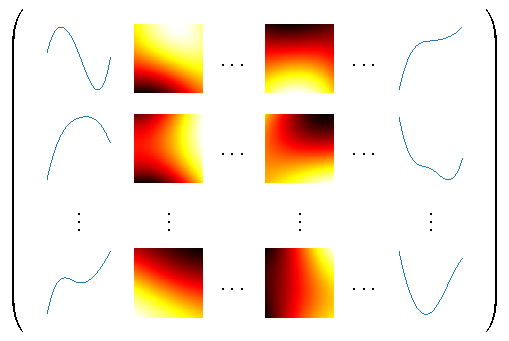
\includegraphics[scale=0.9]{figures/data_matrix.pdf}
    \caption{Functional data matrix, adapted from \cite{berrenderoPrincipalComponentsMultivariate2011}.}
    \label{fig:data_matrix}
\end{figure}

This setting can be generalized to incorporate a general weighting scheme, as \cite{chiouMultivariateFunctionalPrincipal2014} or \cite{happMultivariateFunctionalPrincipal2018a}. We consider the function $\inH{\cdot}{\cdot}_w~:~\HH \times \HH \rightarrow \RR$,
\begin{equation}\label{eq:innerprodH_weight}
    \inH{f}{g}_w \coloneqq \sum_{p=1}^{P} w_p\inLp{\fp}{\gp} = \sum_{p=1}^{P}w_p\int_{\TT{p}} \fp(t_p)\gp(t_p) \dd t_p, \quad f, g \in \HH.
\end{equation}
Let $\Gamma_w : \HH \rightarrow \HH$ denote the weighted covariance operator of $X$, defined as an integral operator with kernel $C$. That is, for $f \in \HH$ and $\pointt \in \TT{}$, the $p$th feature of $\Gamma_w f(\pointt)$ is given by
\begin{equation}\label{eq:covariance_operator_components_weight}
    (\Gamma_w f)^{(p)}(t_p) \coloneqq \inH{C_{p, \cdot}(t_p, \cdot)}{f(\cdot)}_w = \inH{C_{\cdot, p}(\cdot, t_p)}{f(\cdot)}_w, \quad t_p \in \TT{p}.
\end{equation}
Similarly, we define the weigthed inner-product matrix $\mathbf{M}_w$, the matrix of size $N \times N$ with entries
\begin{equation}\label{eq:gram_mat_weights}
    \mathbf{M}_{w, nn^\prime} = \sqrt{\pi_n \pi_{n^{\prime}}}\inH{X_n - \mu}{X_{n^\prime} - \mu}_w, \quad n, n^\prime = 1, \dots, N.
\end{equation}
\begin{remark}
The observation weights $\pi_n$ and the feature weights $w_p$ are not the same and should not be confused. The observation weights are used to give more (or less) importance to specific observations, while the feature weights control for different levels of variation for the features. A discussion on the feature weights is provided in Section~\ref{sub:on_centering_and_reducing}.    
\end{remark}


\subsection{Inference} % (fold)
\label{sub:inference}

If we observe the set $\mathcal{X}$, the ideal estimators of the mean and covariance function are
\begin{equation}\label{eq:perfect_estimator}
    \widetilde{\mu}(\pointt) = \sum_{n = 1}^N \pi_n X_n(\pointt), \quad\text{and}\quad \widetilde{C}(\points, \pointt) =  \sum_{n = 1}^N \pi_n \{X_n(\points) - \widetilde{\mu}(\points)\}\{X_n(\pointt) - \widetilde{\mu}(\pointt)\}^\top, \quad \points, \pointt \in \TT{}.
\end{equation}
Similarly, one could estimate the inner-product $\mathbf{M}$ by replacing the mean by their estimators. The resulting matrix $\widetilde{\mathbf{M}}$ has entries
\begin{equation}\label{eq:perfect_gram_estimator}
    \widetilde{\mathbf{M}}_{nn^\prime} = \sqrt{\pi_n \pi_{n^{\prime}}}\sum_{p = 1}^P \int_{\TT{p}}\{\Xnp(t_p) - \tildemup{p}(t_p)\}\{X_{n^\prime}^{(p)}(t_p) - \tildemup{p}(t_p)\} \dd t_p, \quad n, n^\prime = 1, \dots, N.
\end{equation}
In many applications, the elements of the set $\mathcal{X}$ are observed with error and on a finite grid of points in $\TT{}$. For each $1 \leq n \leq N$, and given a vector of positive integers $\mathsf{M}_n = (\mathsf{M}_n^{(1)}, \dots, \mathsf{M}_n^{(P)})$, let $\mathrm{T}_{n, \mathsf{m}} = (\mathrm{T}_{n, m_1}^{(1)}, \dots, \mathrm{T}_{n, m_P}^{(P)}), 1 \leq m_p \leq \mathsf{M}_n^{(p)}, 1 \leq p \leq P$, be the random observation times for the curve $X_n$. These times are obtained as independent realizations of a random variable $\mathbf{T}$ taking values in $\TT{}$. The vectors $\mathsf{M}_1, \dots, \mathsf{M}_N$ represent an independent sample of an integer-valued random vector $\mathsf{M}$ with known expectation. We assume that the realizations of $X$, $\mathsf{M}$ and $\mathbf{T}$ are mutually independent. The observations associated with an observation $X_n$ consist of the pairs $(Y_{n, \mathsf{m}}, \mathrm{T}_{n, \mathsf{m}}) \in \mathbb{R}^P \times \TT{}$, where $\mathsf{m} = (m_1, \dots, m_P), 1 \leq m_p \leq \mathsf{M}_n^{(p)}, 1 \leq p \leq P$ and $Y_{n, \mathsf{m}}$ is defined as
\begin{equation}\label{eq:model_error}
    Y_{n, \mathsf{m}} = X_n(\mathrm{T}_{n, \mathsf{m}}) + \varepsilon_{n, \mathsf{m}}, \quad 1 \leq n \leq N,
\end{equation}
with the $\varepsilon_{n, \mathsf{m}}$ being independent realizations of a centered error random vector $\varepsilon \in \RR^{P}$ with finite variance $\sigma^2\mathbf{1}_P \in \RR^{P \times P}$ where $\sigma^2 = (\sigma^2_1, \dots, \sigma^2_P) \in \RR^{P}$.

Let $\widehat{X}_n$ be a suitable estimator of $X_n$ applied to the pairs $(Y_{n, \mathsf{m}}, \mathrm{T}_{n, \mathsf{m}})$, such as P-splines \cite[e.g.][]{eilersTwentyYearsPsplines2015} or local polynomials \cite[e.g.][]{fanLocalPolynomialModelling1996}. We define the estimator of the mean function as
\begin{equation}
    \widehat{\mu}(\pointt) = \sum_{n = 1}^N \pi_n \widehat{X}_n(\pointt), \quad \pointt \in \TT{}.
\end{equation}
Concerning the estimation of the covariance of the $p$th feature, we distinguish the diagonal from the non-diagonal points. The estimation of the covariance function of the non-diagonal points is defined as
\begin{equation}\label{eq:cov_estimation}
    \widehat{C}_{p, p}(s_p, t_p) = \sum_{n = 1}^N \pi_n\left(\{\hatXnp{p}(s_p) - \hatmup{p}(s_p)\}\{\hatXnp{p}(t_p) - \hatmup{p}(t_p)\}\right), \quad s_p \neq t_p, \quad s_p, t_p \in \TT{p}.
\end{equation}
The variance function $C_{p, p}(s_p, t_p)$ induces a singularity when estimating the covariance function $C_{p, p}(\cdot, \cdot)$ \cite[see][]{yaoFunctionalDataAnalysis2005,zhangSparseDenseFunctional2016}. We define the estimator of the diagonal of the covariance as
\begin{equation}
    \widehat{C}_{p, p}(s_p, s_p) = \sum_{n = 1}^N \pi_n\{\hatXnp{p}(s_p) - \hatmup{p}(s_p)\}^2 - \sigma_p^2, \quad s_p \in \TT{p}.
\end{equation}
This singularity does not appear in the estimation of the cross-covariance function. We define the estimator of the cross-covariance function between the $p$th and $q$th features by
\begin{equation}
    \widehat{C}_{p, q}(s_p, t_q) = \sum_{n = 1}^N \pi_n\left(\{\hatXnp{p}(s_p) - \hatmup{p}(s_p)\}\{\hatXnp{q}(t_q) - \hatmup{q}(t_q)\}\right), \quad s_p \in \TT{p}, t_q \in \TT{q}.
\end{equation}
The estimator of the inner-product matrix can be defined by replacing the curves by their estimators. Following \cite{benkoCommonFunctionalPrincipal2009} and \cite{grithFunctionalPrincipalComponent2018}, we define the estimator of the inner-product matrix as
\begin{equation}
    \widehat{\mathbf{M}}_{nn^\prime} = \sqrt{\pi_n \pi_{n^{\prime}}}\sum_{p = 1}^P \int_{\TT{p}}\{\hatXnp{p}(t_p) - \widehat{\mu}^{(p)}(t_p)\}\{\widehat{X}^{(p)}_{n^\prime}(t_p) - \widehat{\mu}^{(p)}(t_p)\} \dd t_p, \quad n, n^\prime = 1, \dots, N.
\end{equation}
As for the covariance estimation, the model implies a bias on the diagonal term of the inner-product matrix. A correction for the diagonal of the Gram matrix is given by
\begin{equation}
    \widehat{\mathbf{M}}_{nn} = \pi_n\sum_{p = 1}^P \left\{\int_{\TT{p}}\{\hatXnp{p}(t_p) - \widehat{\mu}^{(p)}(t_p)\}^2 \dd t_p - \sigma_p^2 \right\}, \quad n = 1, \dots, N.
\end{equation}
For the estimation of the variances $\sigma_p^2$, we let the reader refers to \cite{hallVarianceEstimationNonparametric1990} and \cite{hallAsymptoticallyOptimalDifferenceBased1990}.

% subsection inference (end)

% section model (end)